
%author: Ricardo Soto [ricardo.soto@ucv.cl]

\documentclass[11pt]{article}
\usepackage[spanish]{babel}
\usepackage[T1]{fontenc}
\RequirePackage[a-1b]{pdfx}
\usepackage[latin1,utf8]{inputenc}
\usepackage{graphicx}
\usepackage{fancybox}
\usepackage{xcolor}
\usepackage{color}  
%\usepackage[ps2pdf,bookmarks,urlcolor=blue,citecolor=blue,linkcolor=blue,%
%           pagecolor=blue,colorlinks,hyperfigures]{hyperref}

%=============================================================================
% Redefining paragraph

\makeatletter % needed to recognize '@' as a normal char
\renewcommand{\paragraph}{\@startsection{paragraph}{4}{\z@}{-3.25ex \@plus
-1ex \@minus -.2ex}{1.5ex \@plus .2ex}{\normalfont\normalsize\bfseries}}
\makeatother % needed to recognize '@' as a special char
\setcounter{secnumdepth}{4}
\setcounter{tocdepth}{3}

%=============================================================================
% Document

\begin{document}

\renewcommand{\tablename}{Tabla}

\thispagestyle{empty}
\begin{center}
PONTIFICIA UNIVERSIDAD CATÓLICA DE VALPARAÍSO\\
FACULTAD DE INGENIERÍA\\
ESCUELA DE INGENIERÍA INFORMÁTICA\\

\vspace{5cm}

\Large{\textbf{TÍTULO PROYECTO}}

\vspace{3cm}
\normalsize{\textbf{RAMÓN LABBÉ YÁÑEZ}}\\
\end{center}

\begin{flushright}
\vspace{3cm}
INFORME DE AVANCE DE PROYECTO\\
PARA OPTAR AL TÍTULO PROFESIONAL DE\\ 
INGENIERO XXX INFORMÁTICA\\ 
\end{flushright}

\vspace{1cm}
\begin{center} 
MES, AÑO\\
\end{center}

\newpage
\pagenumbering{roman}

%%=============================================================================
%% Abstract


\noindent
\Large{\textbf{Resumen}}\\

\normalsize
El resumen consiste en la presentación clara y concisa de los puntos más
relevantes del trabajo de manera de entregar una idea general del documento. El
resumen antecede la introducción y en los trabajos de título no debe superar las
350 palabras. El contenido del resumen debe estar constituido por una secuencia
de oraciones compuestas y no por una enumeración de tópicos. El primer párrafo
debe presentar el problema principal a abordar. El segundo párrafo debe explicar
la solución desarrollada. El tercer y último párrafo debe presentar los
resultados y conclusiones del trabajo. No deben incluirse fórmulas matemáticas
ni figuras. Después del resumen se deben incluir las palabras claves del
documento.\\

\noindent
\textbf{Palabras Clave:} lenguajes, heurísticas, agentes, patrones de diseño.


\newpage

%%=============================================================================
%% Table of Contents

\tableofcontents
\newpage


%%=============================================================================
%% List of Figures

\renewcommand{\listfigurename}{Lista de Figuras}
\listoffigures
\newpage

%%=============================================================================
%% List of Tables

\renewcommand{\listtablename}{Lista de Tablas} 
\listoftables
\newpage

%%=============================================================================
%% Body of the document

\pagenumbering{arabic}

\section{Introducción}\label{sec:introduccion}
  
La forma en que se escribe y presenta un documento puede incidir de modo
importante en la lectura y comprensión que otros hagan de él. Es por este motivo
que la Escuela de Ingeniería Informática de la Pontificia Universidad Católica
de Valparaíso ha hecho esfuerzos permanentes en la búsqueda de un formato
adecuado para utilizar por parte de los estudiantes en la preparación de
cualquier documento académico que deban presentar en sus asignaturas.

El objetivo de este nuevo formato es estandarizar aspectos generales que sean
aplicables a documentos en distintos contextos, tales como trabajos de
asignaturas~\cite{AptCambridge2003,AptTOPLAS1998}, informes académicos,
trabajos de título, etc...

La Escuela espera que este formato permita mejorar la presentación de los
documentos preparados por sus estudiantes.



  \newpage

 \section{Capítulo 1}\label{sec:cap1}
        Son consideradas figuras: gráficos, diagramas, láminas, fotografías,
esquemas de cualquier naturaleza, dibujos, planos, organigramas, flujogramas,
cuadros y tablas tanto en color como blanco y negro...

\subsection{Presentación Gráfica}
       
Un ejemplo es la figura~\ref{fig:pucv}....


\begin{figure}[!htbp]
\begin{center}
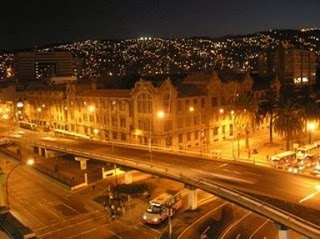
\includegraphics[width=0.6\linewidth]{imagenes/pucv.jpg} 
\caption{Edificio PUCV.}\label{fig:pucv}
\end{center}
\end{figure}
   \newpage

 \section{Capítulo 2}\label{sec:cap2}
   

\subsection{Tablas}

Los resultados se muestran en la tabla~\ref{table:resultados}...

\begin{table}[htbp!]
\begin{center}
\begin{tabular}{|l|l|l|l|l|l|l|l|}
\hline
Valores    & a & b & c & b & e  & f & g \\
\hline
Tipo 1     & 5 & 4 & 0 & 2 &  4 & 5 &  1  \\
Tipo 2     & 1 & 3 & 0 & 3 &  8 & 9 &  9  \\
Tipo 3     & 2 & 2 & 1 & 0 &  7 & 8 &  3  \\
Tipo 4     & 6 & 2 & 1 & 0 &  5 & 8 &  2  \\
\hline
\end{tabular}
\end{center}
\caption{Resultados\label{table:resultados}}
\end{table}

\subsection{Ecuaciones}

La ecuación~\ref{ec:smoothing-1} muestra...

\begin{equation} \label{ec:smoothing-1}
 {f_i}_1 (S_j) = x_{0}
\end{equation} 


\begin{equation} \label{ec:smoothing-2}
 {f_i}_n (S_j) =  x_{n-1} + \beta_i {f_i}_{n-1} (S_j)
\end{equation} 
   \newpage


%%=============================================================================
%% Biblio

\bibliographystyle{plain}
%\bibliographystyle{alpha}
\bibliography{bibliography}	


\end{document}